\documentclass[conference]{IEEEtran}
\IEEEoverridecommandlockouts
% The preceding line is only needed to identify funding in the first footnote. If that is unneeded, please comment it out.

\makeatletter
\def\lst@makecaption{%
  \def\@captype{table}%
  \@makecaption
}
\makeatother

\newcommand{\tool}{\textsc{BadUSB-C}\xspace}

\newcommand{\outline}[1]{\mytodocyan{[outline: #1]}}
\newcommand{\mytodocyan}[1]{\textcolor{cyan}{\ding{46}~{\sf}~#1}}


\newcommand{\hongyi}[1]{\mytodopink{[hongyi: #1]}}
\newcommand{\mytodopink}[1]{\textcolor{violet}{\ding{46}~{\sf}~#1}}

\newcommand{\shuqing}[1]{\mytodopurple{[shuqing: #1]}}
\newcommand{\mytodopurple}[1]{\textcolor{purple}{\ding{46}~{\sf}~#1}}

\newcommand{\yechang}[1]{\mytodored{[yechang: #1]}}
\newcommand{\mytodored}[1]{\textcolor{red}{\ding{46}~{\sf}~#1}}

\newcommand{\linyou}[1]{\mytodoblue{[linyou: #1]}}
\newcommand{\mytodoblue}[1]{\textcolor{blue}{\ding{46}~{\sf}~#1}}

\newcommand{\chaozu}[1]{\mytodogrey{[chaozu: #1]}}
\newcommand{\mytodogrey}[1]{\textcolor{gray}{\ding{46}~{\sf}~#1}}
\usepackage{enumerate}
\usepackage[shortlabels]{enumitem}

\newcommand{\fengwei}[1]{\textcolor{cyan}{fengwei: #1}}

\newcommand{\mycircled}[1]{%
	\begin{tikzpicture}[baseline={(char.base)}]
		\node (char) {\small{#1}};
		\node[draw,circle,minimum size=10,inner sep=0pt,overlay] (char.center){};
	\end{tikzpicture}
}
\usepackage{textcomp}

\usepackage{tikz,pgf}
\usetikzlibrary{calc}
\makeatletter
\def\mfontsize{\f@size}
\newcommand{\circled[2]}{
	\tikzset{mystyle/.style={circle,#1,minimum size=10,inner sep=0pt}}
	\tikz[baseline=-3pt]
	{
		\node[mystyle] (char.center) {\vphantom{WAH1g}#2};
	}
}
\makeatother

\definecolor{myyellow}{RGB}{237,125,49}
\definecolor{myblue}{RGB}{91,155,213}

\usepackage[breaklinks=true,hidelinks,colorlinks=true,citecolor=blue,urlcolor=black,linkcolor=black]{hyperref}

\usepackage{xspace}
\usepackage{cite}
\usepackage{amsmath,amssymb,amsfonts}
\usepackage{graphicx}
\usepackage{textcomp}
\usepackage{xcolor}
\usepackage{hyperref}
\usepackage{threeparttable}
\usepackage{colortbl}
\usepackage{graphicx}
\usepackage{listings}
\usepackage{color}
\usepackage{array}
\usepackage{float}
\usepackage{graphicx}
\usepackage{subfigure}
\usepackage{multirow}
\usepackage{colortbl}
\usepackage[linesnumbered,boxed]{algorithm2e}
\usepackage{algpseudocode}
\usepackage{framed}
\setlength\FrameSep{0.5em}
\usepackage{pifont}
\usepackage{enumitem}
\usepackage{balance}
\usepackage{url}
\usepackage[T1]{fontenc}
\usepackage[utf8]{inputenc}
\usepackage[font=small,labelfont=bf,tableposition=top]{caption}
\usepackage{booktabs}
\usepackage{tabularx}
\usepackage{diagbox}
\usepackage{algpseudocode}
\usepackage{amsmath}
\usepackage{listings}
\usepackage{makecell}

\lstset{
	frame=single,
	breaklines,
	language=python,
	basicstyle=\small,
}


\def\BibTeX{{\rm B\kern-.05em{\sc i\kern-.025em b}\kern-.08em
    T\kern-.1667em\lower.7ex\hbox{E}\kern-.125emX}}


\begin{document}

\title{\tool: Revisiting BadUSB with Type-C}

\author{\IEEEauthorblockN{1\textsuperscript{st} Given Name Surname}
\IEEEauthorblockA{\textit{dept. name of organization (of Aff.)} \\
\textit{name of organization (of Aff.)}\\
City, Country \\
email address or ORCID}
\and
\IEEEauthorblockN{2\textsuperscript{nd} Given Name Surname}
\IEEEauthorblockA{\textit{dept. name of organization (of Aff.)} \\
\textit{name of organization (of Aff.)}\\
City, Country \\
email address or ORCID}
\and
\IEEEauthorblockN{3\textsuperscript{rd} Given Name Surname}
\IEEEauthorblockA{\textit{dept. name of organization (of Aff.)} \\
\textit{name of organization (of Aff.)}\\
City, Country \\
email address or ORCID}
\and
\IEEEauthorblockN{4\textsuperscript{th} Given Name Surname}
\IEEEauthorblockA{\textit{dept. name of organization (of Aff.)} \\
\textit{name of organization (of Aff.)}\\
City, Country \\
email address or ORCID}
\and
\IEEEauthorblockN{5\textsuperscript{th} Given Name Surname}
\IEEEauthorblockA{\textit{dept. name of organization (of Aff.)} \\
\textit{name of organization (of Aff.)}\\
City, Country \\
email address or ORCID}
\and
\IEEEauthorblockN{6\textsuperscript{th} Given Name Surname}
\IEEEauthorblockA{\textit{dept. name of organization (of Aff.)} \\
\textit{name of organization (of Aff.)}\\
City, Country \\
email address or ORCID}
}

\maketitle
\thispagestyle{plain}
\pagestyle{plain}


\begin{abstract}
\outline{Brief intro of USB protocol}\\
\outline{Brief intro of Rubber Ducky}\\
\outline{What have we done, our contribution}\\
\outline{Our experiment/case study, Attack of shops}\\
\end{abstract}


\begin{IEEEkeywords}
USB;BadUSB
\end{IEEEkeywords}



\section{Introduction}
\label{sec:introduction}
\noindent\outline{Intro of USB protocol}\\
\outline{Rubber Ducky and its limitation}\\
\outline{Bank Robber and its function, out contribution}\\
\outline{Case Study of QR Scanning}\\
\section{Background}
\label{sec:background}
%\shuqing{Maybe we could introduce HID devices somewhere.}
%\noindent\outline{USB Standard}\\

We first introduce the development of USB specification and emphasize the key
points adopted in this work. We also organized a brief timeline for introducing
key points of each protocol in Table~\ref{table:usb_timeline}.

%\noindent\outline{USB1.x}\\
Proposed in 1996, USB 1.0~\cite{usb10} was developed to provide a unified
interface and thus reducing the cost of reconfiguring the software. It is
worth mentioning that as a polled-bus interface, all data transfers are
initiated by the host.

%\noindent\outline{HID Protocol}\\
Right after one year of the appearance of USB 1.0, a standard named HID (Human
Interface Device)~\cite{hid} was born based on USB. HID is
designed with to unify the implementation for devices like mice,
keyboards, etc. Before its appearance, the standard is divided between
manufacturers, for example, the mouse of Company A may use X-Y coordinates to
represent its location while the mouse of Company B uses relative displacement.
This means every device needs its own driver to work. After HID, users only need to
write one driver for an entire class of HIDs. Furthermore, HID standard also
requires all devices to be PnP (\emph{Plug-and-Play}), which is indeed
convenient but insecure too.

In 1998, the first widely supported USB protocol was born. USB1.1~\cite{usb11}
provided two data transfer rates which are low speed (1.5 Mbit/s) and full
speed (12 MBit/s). At this point, due to the transfer limit, it only supports
limited types of devices like keyboards, mice, etc.

%\noindent\outline{USB2.0}\\
In 2000, USB 2.0~\cite{usb20} specification was released. With high speed \mbox{(480
Mbit/s)} mode introduced, printers, cameras, CD-ROM drives, and network cards were
supported in this revision. Such a high data transfer rate also gave rise to the
popularity of ``flash drive'', a portable device that allows physically
transferring data around~\cite{sok}. Though various peripherals were supported
in USB 2.0, there was no reliable way to identify the type of device. This
security flaw allowed attacks like BadUSB~\cite{badusb,rubber}.

%\noindent\outline{USB3.x}\\
USB 3.0~\cite{usb30} was announced in 2008, with a super speed (5 Gbit/s) data
transfer rate. Like its predecessor, more classes of peripherals were supported
in this revision. In 2013, the USB Type-C connector standard was introduced as a
part of USB 3.1~\cite{usb31}, providing a unified connector type for
PowerDelivery (PD), Thunderbolt, DisplayPort, and HDMI.  Yet no improvement of
security was introduced in 3.x revisions, meaning any device claiming
itself as a monitor can capture the video stream from the host. Exposing
such a multi-propose connector unprotected is insecure and allows attacks like
this work \tool. In 2017, USB 3.2~\cite{usb32} was released, doubling the data
transfer rate (20 Gbit/s).

%\noindent\outline{Connector Standard}
\begin{figure}[t]
    \centering
	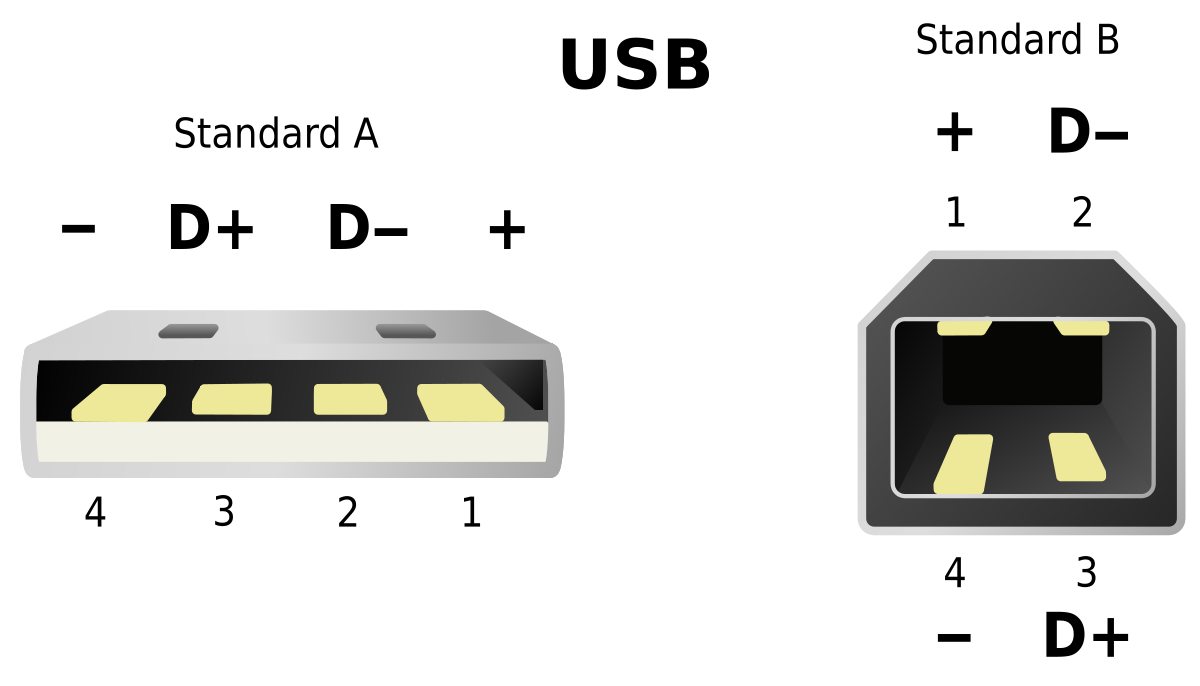
\includegraphics[width=0.7\linewidth]{./Figs/usb_conn.png}
	\caption{USB 1.x \& 2.x Connector.}
	\label{fig:usb_conn}
\end{figure}

As illustrated in Figure~\ref{fig:usb_conn}, the original USB 1.x \& 2.x
connector only has two pins for data transferring \mbox{(D+ \& D-)}, which has
significantly limited data transfer rate \mbox{(5 Gbits/s Max)} and cannot support for
peripherals like DisplayPort \mbox{(10.8 Gbit/s Min)}. Apart from that, support for
other peripherals also require dedicated transferring lane as their standards
are not compatible with USB in most cases.  

\begin{figure}[t] 
	\centering
	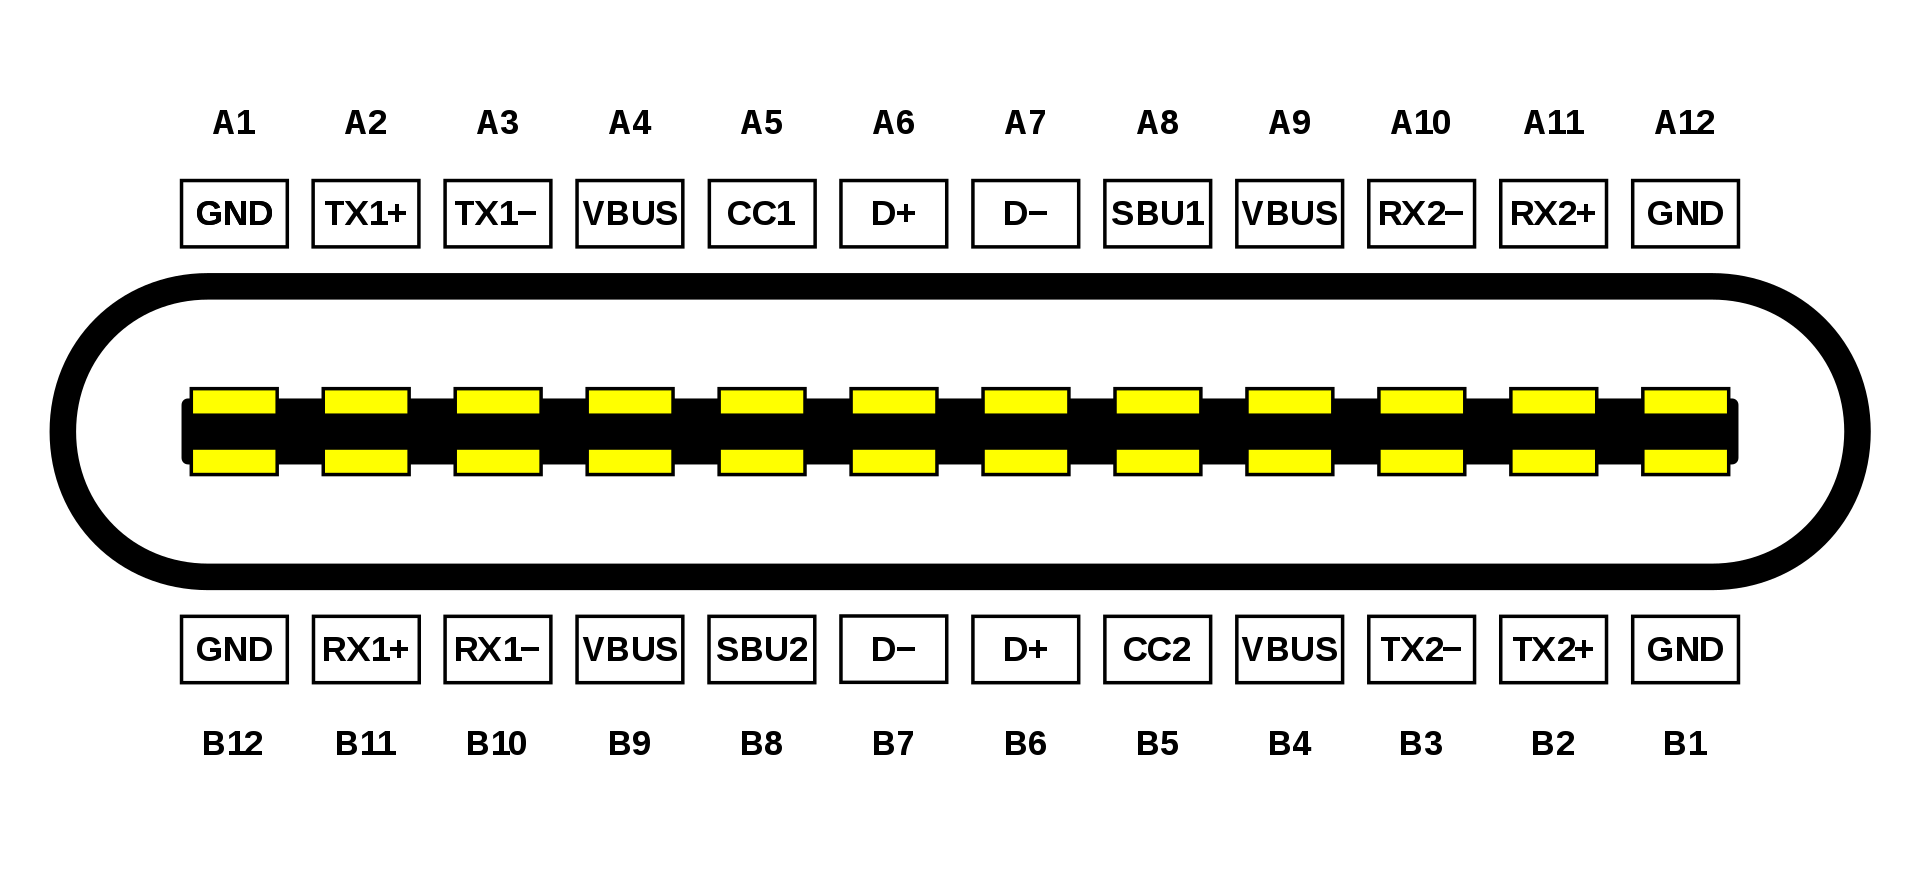
\includegraphics[width=\linewidth]{./Figs/usb_c_conn.png} 
	\caption{USB Type-C Connector.} 
	\label{fig:usb_c_conn} 
\end{figure}

Thus, to provide support towards a wider range of peripherals, a 24-pins
standard called USB Type-C~\cite{typec} is introduced in 2013 by USB-IF~\cite{usbif}. As it is designed to be double-sided, the number of actually usable
pins is halved. Nevertheless, this standard has largely enhanced the capability
of the USB 3.x protocol. As presented in Figure~\ref{fig:usb_c_conn}, Type-C added
two high-speed data lanes \mbox{(TRX1 \& TRX2)} and kept the original data lane \mbox{(D+ \&
D-)}. The added lanes are used exclusively to support peripherals like
DisplayPort while the kept data lane transfers USB packets.

%\noindent\outline{Security Problem}\\
During the development of USB specification, security was rarely considered. As
the USB-IF believes it is the duty of original equipment manufacturers \mbox{(OEMs)}
to decide whether security features should be implemented~\cite{usbsec}. But the divergent implementations give a chance for attacks like
BadUSB~\cite{rubber} and our \tool.

%\fengwei{FIXME: add a reference for each attack in the Table.}
%\fengwei{FIXME: The table is too wide, exceeds the max size.}
\begin{table*}
\begin{tabular}{|c|l|c|c|c|}
	\hline
	\textbf{Year} & \textbf{Protocol Version} & \textbf{Supported Peripherals} & \textbf{Transfer Speed} & \textbf{Attacks} \\
	\hline
	1996 & USB 1.x~\cite{usb10,usb11} & Keyboard, Mouse... & 1.5 Mbit/s or 12 Mbit/s & HID Emulating (BadUSB)~\cite{badusb} \\
	\hline
	2000 & USB 2.0~\cite{usb20} & Flash Drive, High-Definition Link, CD Driver... & 480 Mbit/s & Autorun Attack~\cite{duqu}, Juice Filming~\cite{JFC,JFCImpact} \\
	\hline
	2008 & USB 3.0~\cite{usb30} & / & 5 Gbit/s & / \\
	\hline
	2013 & USB 3.1~\cite{usb31} & HDMI, DisplayPort, ThunderBolt... & 10 Gbit/s & \tool \\
	\hline
	2017 & USB 3.2~\cite{usb32} & / & 20 Gbit/s & / \\
	\hline
\end{tabular}
	\linebreak
\caption{USB Protocol Timeline.}
\label{table:usb_timeline}
\end{table*}

\section{Related Work}
\label{sec:related_work}
%\hongyi{Move the stuff about USB protocol to Background}\\
%\outline{Attack based on USB 1.0, briefly}\\
%\outline{Attack based on USB 2.0, focus on works about application and transport layer}\\
%\outline{Attack survey table}\\
%\outline{Attack or current works about USB Type-C}\\

In this part, we survey related works on USB attack in Section~\ref{subsec:usb_attack}, and USB defence security in Section \ref{subsec:usb_defence}, respectively.

\subsection{USB Attack}
\label{subsec:usb_attack}
\chaozu{DoS(Fuzzing), Code injection, HID emulation, JFC, our work}
During the development of USB protocol, there are many USB-based attacks were proposed, ranging from DoS (denial of service) to protocol masquerading. Here we will introduce them following an order of their category.\hongyi{What?}

From the kernel perspective, its USB software stack generally expects devices to follow the USB standard and may not consider corner cases of malformed USB packets. Based on this, Facedancer\cite{facedancer} and Syzkaller\cite{syzkaller} uses fuzzing technique to uncover the bugs lying in the kernel drivers. These bugs can cause kernel crash and lead to a DoS situation. Though this poses a great challenge to the availability of a system, this attack still requires physical access to the host and is unable to cause more damage other than DoS.

In the field of USB security, protocol masquerading is also a widely used attack scheme. Due to the lack of authentication in USB protocol, malicious devices can hide their real functionality with re-written firmware\cite{rubber,badusb, rubberducky2020, usbbypassing, iseeyou, usbdriver}. These works rewrite the firmware of a normal-looking flash drive, which allows it to pretend as other devices. When these modified drives are connected to the host, they will be recognized as keyboard or mouse. Then the attacker can execute malicious payloads as they were using the victim's devices. But due to the limitation of USB 2.0\cite{usb20} protocol, these BadUSB attacks are unable to obtain video feedback from the victim as video were not supported until USB 3.0 \cite{usb30}. Though USB 2.0 does not support video transmission, there exists a protocol called MHL(Mobile High-Definition Link) which extends the USB standard and allow video signal to be transmitted through USB interface. JFC\cite{JFC}, short for juicy filming charging is such a work which abuses this standard and exfiltrate video data from victim without permission. But in JFC, this data exfiltration is not combined with BadUSB attacks and MHL is an outdated standard, which limits its capability.

Besides attacking from the protocol perspective, there are works trying to use USB device as a payload delivery means. Duqu\cite{duqu} uses a user-mode rootkit to hide malicious files on the USB storage device, \cite{flame} uses a zero-day exploit and malicious \textit{autorun.inf} to execute the malware automatically. There are also works like \cite{brain, stuxnet, conficker} following the same paradigm and performing code-injection attacks. These attacks are much more damaging and flexible comparing to those previous ones, but they requires certain existing flaw like \cite{zero-day} and USB are merely a payload delivery method.

As a data transmission protocol, USB inevitably leaks electromagnetic signals to the environment which may contains sensitive information. Leveraging this physical phenomenon, there are works like \cite{smartphone, poweremi,revealing,su2017usb, usbgpslocator, bates2014leveraging, badusbhub, usbfinger, side, usbdriver} eavesdropping leaked signals and recovering the sensitive data. In a similar fashion, \cite{usbee, turnip} emit electromagnetic emissions by data injection on the bus with the connected USB devices as a RF transmitter and \cite{usbkiller, cable} inject analog power to cause physical damage to the host machine. Even though the data, including the video data, could be recovered in this way, these attacks for executing malicious code is too difficult to work, and the invisibility is a problem cannot be ignored due to the spacial locality of radio frequency. 

Since USB 3.1 was introduced with USB Type-C in 2013, display port and HDMI connectors have been provided by USB Type-C, transferring of video data can be combined with the other attacks, like protocol masquerading,  protocol corruption and code injection. This has paved the path for our \tool.




\chaozu{attack table}\\
\chaozu{enum diagram}


\subsection{USB Defence Security}
\label{subsec:usb_defence}
There are already many defenses proposed against BadUSB attacks and a comprehensive investigation of previous work.\cite{sok}.

From the hardware perspective, BadUSB attack requires `D-' and `D+' pins which are defined by protocol to transmitting data.
Without these pins, data can't be transferred via USB cable. Based on this fact, USB Condom \cite{Condom} is a hardware solution to block data channel by adding blocker in the connector. This blocker can cut off the `D-' and `D+' connection while leave power pins intact.
However, this method poses a great challenge to plug-and-play property of USB, as once it is deployed, it will stop all USB functions other than charging. 

Under the premise of ensuring the full functionality of USB devices, there have been some works trying to improve the security during connection establishment.
Windows Defender ATP\cite{windenfenderwhite} maintains a whitelist of USB devices, only devices on the whitelist are allowed to communicate with the host. This prevents all potential attacks from untrusted devices. But this requires users to have a certain safety awareness and technical background to maintain a valid whitelist. For example, a naive user may add the USB device from unknown sources to his/her whitelist without precaution. There are designs can overcome this drawback. For instance, Mohammadmoradi et al\cite{mohammadmoradi2018making} proposes a strategy to generate such a whitelist automatically. This strategy first generates a unique fingerprint for each device based on its functionality. Then these fingerprints are used to maintain a safe and valid whitelist of USB devices. There is another work mediating USB connectivity for Industrial Control. TMSUI\cite{yang2015tmsui} relies on rich experience of administrators to build a whitelist. However, some modified USB devices may hide their real functionality from the user.

To solve this flaw, GoodUSB\cite{tian2015defending} will report the functionality claimed by the device to user and let user decides whether to authorize. When a device is plugged in, GoodUSB will load its driver but limit its functionality until a series of authorizations is completed. These authorizations are designed to be performed manually. As BadUSB is normally unable to obtain the video stream of the host, it is impossible for an attacker to complete these authorization with automatic script. Thus this defense is sufficient for normal BadUSB attack. But if the attacker has the access to victim's screen, GoodUSB will be bypassed easily as the attacker can just complete these authorization manually and perform subsequent attacks.

After the USB enumeration and driver loading, there are also works trying to archive `defense in depth' against BadUSB attack.
Neuner et al.\cite{neuner2018usblock} prevents BadUSB attacks from malicious flash drive by analyzing the temporal characteristics of BadUSB-like attacks. This defense mechanism is effective because the attacker cannot obtain the screen of the host using just BadUSB. In this case, the malicious device can only inject key stoke in a very short time to reduce the risk of being discovered. This defect causes the typing characteristics of BadUSB to be detectable.  Pham et al. \cite{pham2010optimizing} optimizing windows security features. It can block the execution of unsigned files, the installation of unsigned driver carried on portable media. What's more, in GoodUSB, a VM is deployed in host to as a honeypot to detect and stop malicious behavior of USB devices. 

In addition to injection attacks, data theft attack is also one of the focuses of academic community. As mentioned in Section~\ref{subsec:usb_attack}, there exist an attack called JFC (juicy film charging)\cite{JFC} which abuses the MHL standard to steal video stream from the victim. In order to mitigate this issue, Meng et al proposed a statistical model using status like GPU/CPU usage to detect JFC attack\cite{meng2018252}.

To summarize, there exists a clear trade-off between the effectiveness and the plug-and-play property. Though hardware disabling solution like USB Condom archives the almost absolute security, the functionality of USB is scarified. Other solutions like GoodUSB or whitelist are either bypassable or insufficient under certain cases. 
Some vendors may sacrifice defensive capabilities to improve usability, which allows attackers to take advantage of.

We summarize the former effort in USB attack and defense in Table~\ref{table:attack_vs_defense}, which illustrates the effectiveness of each defense against various attacks including our \tool.
\begin{table*}
	\centering
	\begin{tabular}{|c|c|c|c|c|c|c|}
		
		
		\hline
		\diagbox[width=1.46in] {Defence}{Attack} & Rubbery Ducky\cite{rubber}, \cite{rubberducky2020},USBderivery\cite{usbdriver} & Duqu\cite{duqu} & JFC\cite{JFCImpact}&\cite{smartphone}\cite{poweremi} and \cite{usbdriver}& Armory\\
		
		\hline 
		USB condom \cite{Condom}& Yes & Yes & Yes & Yes & Yes\\
		\hline 
		Pham et al. \cite{pham2010optimizing}, odix\cite{OLEA}& No & ? & No & No & No\\
		\hline 
		TMSUI\cite{yang2015tmsui}& No & Yes? & No & No & No\\
		\hline 
		Windows Defender ATP\cite{windenfenderwhite}& No & Yes? & No & No & No\\
		\hline 
		GoodUSB\cite{tian2015defending}& Yes & Yes & Yes? & No & No \\

		\hline
		Neuner et al.\cite{neuner2018usblock}& Yes & No & No & No & depends? \\
		\hline
		Meng et al\cite{meng2018252}& No & No & Yes & No & ?\\
		\hline
	\end{tabular}
	\linebreak
	\caption{Effectiveness of defense against different attacks}
	\label{table:attack_vs_defense}
\end{table*}





\section{\tool}
\label{sec:badusb}
\subsection{Threat Model}

We build our threat model on the basic assumptions that common users without
technical background would not treat normal-looking USB device as malicious and be cautious about them. This assumption is consistent with existing works~\cite{JFCImpact}. Moreover, we neglect the
effect of notifications from USB devices, as users may not have the knowledge to fully understand such notifications. In
fact, during our experiment, no device had security notifications raised about
suspicious USB devices and only mobile devices had raised a charging notification
about our \tool, which may not be a sufficient warning for users.

We also assume the victim's device is equipped with fully functional USB 3.x
protocol and USB Type-C connector. As the USB 3.x standard is
common nowadays, this assumption can be easily fulfilled especially in recent
devices.

%\subsection{Motivation}
%\noindent\outline{Limitation of Rubber Ducky}\\
%\outline{Our functionality different mode listing?}\\
%\hongyi{The following mode is to be further decided}
%\outline{Automatic Scripting Mode}\\
%\outline{Remote Control Mode}\\
%\outline{OCR/QR Recognition Mode}\\

\subsection{Implementation}
%\noindent\hongyi{The following mode is to be further decided}\\
%\outline{DETAIL of each mode}\\ \outline{Automatic Scripting Mode}\\
%\outline{Remote Control Mode}\\ \outline{OCR/QR Recognition Mode}\\

As introduced in Section~\ref{sec:related_work}, 
existing works~\cite{rubber,badusb,
rubberducky2020,usbbypassing,iseeyou,usbdriver} focus on BadUSB attacks.
Many of these take advantage of the \textit{trust-by-default} policy of PC,
pretend to be normal HID devices and utilize USB protocol to perform attacks.
However, these attacks suffer from various drawbacks: \ding{182} attackers can
only simulate limited types of devices such as HIDs (like keyboards and mice)
and disks, which makes the attacks less effective; \ding{183} accurate attacks
could not be performed due to lack of user interface (UI) status. Whatever HID the
attackers simulate their USB devices to be, they could not obtain the UI to
check the status information, which makes it nearly impossible to carry out
their attacks precisely or know the effects after attacks.

%Though BadUSB devices\cite{badusb} like Rubber Ducky\cite{rubber,
%rubberducky2020} emulates as a HID device enabling various arbitrary execution
%attacks, fetching feedback from the victim is much more limited.
Based on the drawbacks introduced above, several defense mechanisms were
proposed. GoodUSB~\cite{tian2015defending}
implemented a CAPTCHA-like~\cite{captcha} procedure, which requires user to
complete certain challenges when an unknown HID device is plugged in. As the
BadUSB is only able to emulate a limited kind of devices such as HIDs or disks, by
no means the BadUSB can bypass it. 

In this work, we utilize the new features of USB 3.x~\cite{usb31,usb32} to
address the problem above.  Benefiting from the latest protocol, we simulate
external display and thus obtain the video stream to perform accurate
attacks.
Thus, our \tool is capable of
bypassing defenses such as GoodUSB. Taking advantage of USB 3.x~\cite{usb31,usb32},
\tool can fetch the video stream of the victim and complete the challenge
manually by the attacker. Moreover, with video capability combined with
traditional BadUSB, our \tool achieved multiple new attack paradigms and are
tested under various real-world scenarios.

As there were various BadUSB implementations available, this work focuses on our new extensions. Next, we first introduce the
components we used in \tool, then we focus on the three different attack modes
we implement for various scenarios.

\subsubsection{Attack Model}


Figure~\ref{fig:attack_model} shows the architecture of our attack model. \mycircled{1} represents the victim's devices; \mycircled{2} is our \tool; \mycircled{3} is the attacker's remote PC. The details of each component in \tool are as follows.\mycircled{1} 

%\fengwei{We need to
%explain the figure. What are the boxes? Where is victim? Where is the attacker?
%The list below only shows the internal components in the malicious USB device.
%We might also consider to explain this in the Figure caption.}

\begin{itemize}
	\item\textit{USB 3.x Hub} exports the USB 3.x connector into various ports, like DisplayPort, USB 2.0 port etc.
	\item\textit{Video Capture Card} convert DisplayPort signal into UVC-compatible\hongyi{citation needed} data, which is later processed by embedded computer.
	\item\textit{Single Board Computer} processes video stream from the victim where private data is extracted and transmitted via GSM/WiFi to the attacker.
	\item\textit{HID Emulator} emulates HID device which can be controlled from the attacker.
\end{itemize}


\begin{figure}[t]
	\centering
	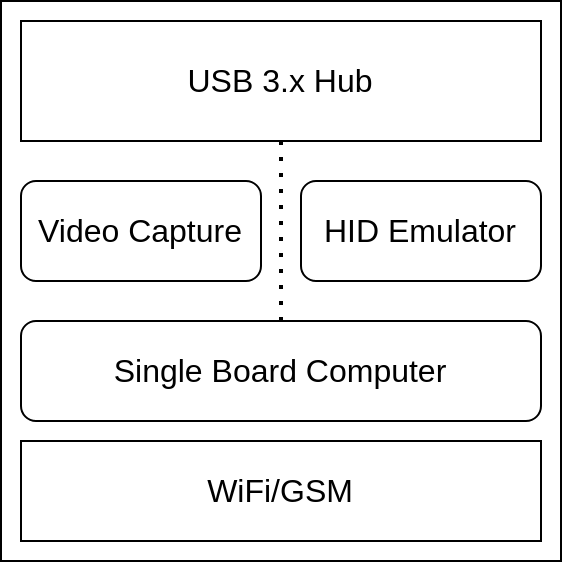
\includegraphics[width=\linewidth]{./Figs/attack_model.png}

	\begin{tabular}{ll}
<<<<<<< HEAD
	\mycircled{1}Victim's Device    &\mycircled{2}\tool\\
	\mycircled{3}Attacker's Device
=======
	\mycircled{1} Victim's Devices    &\mycircled{2}\tool\\
	\mycircled{3} Attacker's Remote PC
>>>>>>> 7bce229ca8ea38c7e1f77ea6f0bbd26f20727864
	\end{tabular}

	\caption{Attack Model}%\shuqing{Need to be more compact.}
	\label{fig:attack_model}
\end{figure}

\textbf{Scripting Mode.} This mode majorly relies on the ``HID Emulator'' to
send constructed HID packet to the victim. These constructed HID packets are
interpreted by the victim as valid keystrokes and mouse moves. Thus, the
attacker can executes arbitrary scripts on the victim's device. This is the
function of the original BadUSB. Based on this, we made the following
improvement.

First, \tool supports defense-bypassing. As the original BadUSB cannot get
feedback from the victim, defense mechanisms like GoodUSB
\cite{tian2015defending} are sufficient to prevent these BadUSB attacks.
However, these defense mechanisms leverage visual notification to block access
for unknown USB devices. This means that when the defense request authorization
from the user, our \tool is able to capture the content of authorization
challenge and bypass it. After the defense is bypassed, \tool continues the
emulation and script execution, resulting in a successful attack.

Moreover, as the mouse relies on the visual feedback to work properly, its
emulation and automation were not supported by the original version of BadUSB.
Yet with the video output support from USB 3.x, our \tool implements
full-functional mouse emulation. This function enables attacks toward pure GUI
programs and shows great potential in the mobile attack scenario. Details can
be obtained in Section~\ref{sec:experiment}.

The advantage of this mode is that it archives defense bypass and attack
feedback with video streaming.  \fengwei{I don't understand the sentence below.}\hongyi{Fixed, I think it's redundant and less important}
%As mentioned above, we only require video stream at the beginning (defense
%bypass) and the end (result feedback) of the attack.
Moreover, with mouse
supported, \tool extends the original BadUSB attack surface and perform well in
mobile device.

\textbf{Privacy Extraction Mode.} \tool under this mode does not emulate other
USB device and solely relies on the video stream function of USB 3.x; it uses
``Video Capture'' component to transmit the stream to embedded ``Single Board Computer''\fengwei{What is embedded computer? Do we define this in the previous\hongyi{Fixed by using the term mentioned in Figure}
text?}. The victim's device would mistakenly treat \tool as an external monitor
and output its video stream. This stream is latter processed by the embedded
computer to extract private data.

When running in this mode, \tool passively processes the victim's video stream
and detect for ``valuable'' private data.  The data is considered as
``valuable'' or not is decided by a customized detector, we implement a simple
payment code detector for the demonstration purpose. Though this detector is
simple to implement, we successfully transfer money from the victim to the
attacker. More detail can be obtained in Section~\ref{sec:experiment}.

It is worth mentioning that \tool under this mode is completely passive, making
it hard to be detected and defended. With different detector implemented, \tool
under this mode is capable of serving more purposes.

\textbf{Remote Control Mode.} In \tool, we have implemented all components
required to control a computer/mobile device remotely, including a video stream
and a keyboard/mouse emulation. Thus with all components enabled, not only will
the victim's device treat \tool as an external display, but also a valid HID
input source. Hence we can archive complete hijack of victim's device.

\tool under this mode follows a simple logic. \tool will receive video stream
from the victim's device and redirect it to the attacker via GSM/WiFi. In the
meanwhile, \tool also receives keystrokes and mouse movement from the attacker
through GSM/WiFi and replay them to the victim by the USB emulation.

This mode enable attacker to perform delicate operation that is beyond
automation. Moreover, this mode provides a backdoor that does not require host
network and thus is undetectable by the firewall running on the host machine.
%\hongyi{I think this is a quite good selling point?}\shuqing{Agree with
%Hongyi.}

The advantage of this mode is that it can completely hijack the victim device
and provide a backdoor beyond detection of firewalls. But this complete control
also comes with the price of high power consumption and risk of being detected
by the user.


\section{Experiment}
\label{sec:experiment}
%\shuqing{Many parts in this section are much more likely to lie in implementation, introducing how \tool works. Doesn't look like experiment.}

%\shuqing{Experiment for devices and case study needed.}

To evaluate the effectiveness of \tool in different modes, we conducted three
experiments on \tool using devices with USB Type-C capabilities from different
OEMs, including a mobile phone, a tablet, and a laptop.

\textbf{Setup.} 
%\fengwei{I would suggest to add references for devices such as
%Pi, ATMEGA32U4 board, Yamazawa, etc.} 
As mentioned in Section~\ref{sec:badusb},
our \tool only requires common components that are easily accessible online or
in any electronic store. Here we choose the following parts to build a
prototype. To begin with, we choose the Raspberry Pi 4B~\cite{pi4b} as the embedded Single Board 
Computer inside \tool, which is powerful enough to process video data and has
an onboard WiFi chip. As for the HID Emulator, we use an Atmel ATMEGA32U4 board~\cite{atmel}
with USB protocol support, which is able to emulate multiple HID devices
with our modified firmware. About the USB 3.x Hub, we use one from the
UGREEN~\cite{ugreen}, which supports HDMI, USB 2.0, and many other exported peripherals.
Apart from these essential parts, we also use an auxiliary power-bank to
provide power for the Raspberry Pi and the mobile devices used by the victim.
The image of our \tool prototype can be found in Figure~\ref{fig:armory}.
\mycircled{A} is a Huawei mobile phone as the victim's device; \mycircled{B} is a compact look of \tool prototype; \mycircled{1} is the USB 3.x Hub; \mycircled{2} is a Raspberry Pi 4B as the Single Board Computer; \mycircled{3} is an auxiliary power bank; \mycircled{4} is the Video Capture Card; \mycircled{5} is an Atmel ATMEGA32U4 board as the HID Emulator. 
%\fengwei{We need to explain the Figure. What is "A"? What is "B", Where are 1,
%2, 3, 4, and 5?}\hongyi{Is the caption sufficient? If explain here, I feel quite redundant}
\fengwei{I think it is necessary to explain them in the text again.}


\begin{figure}[t]
	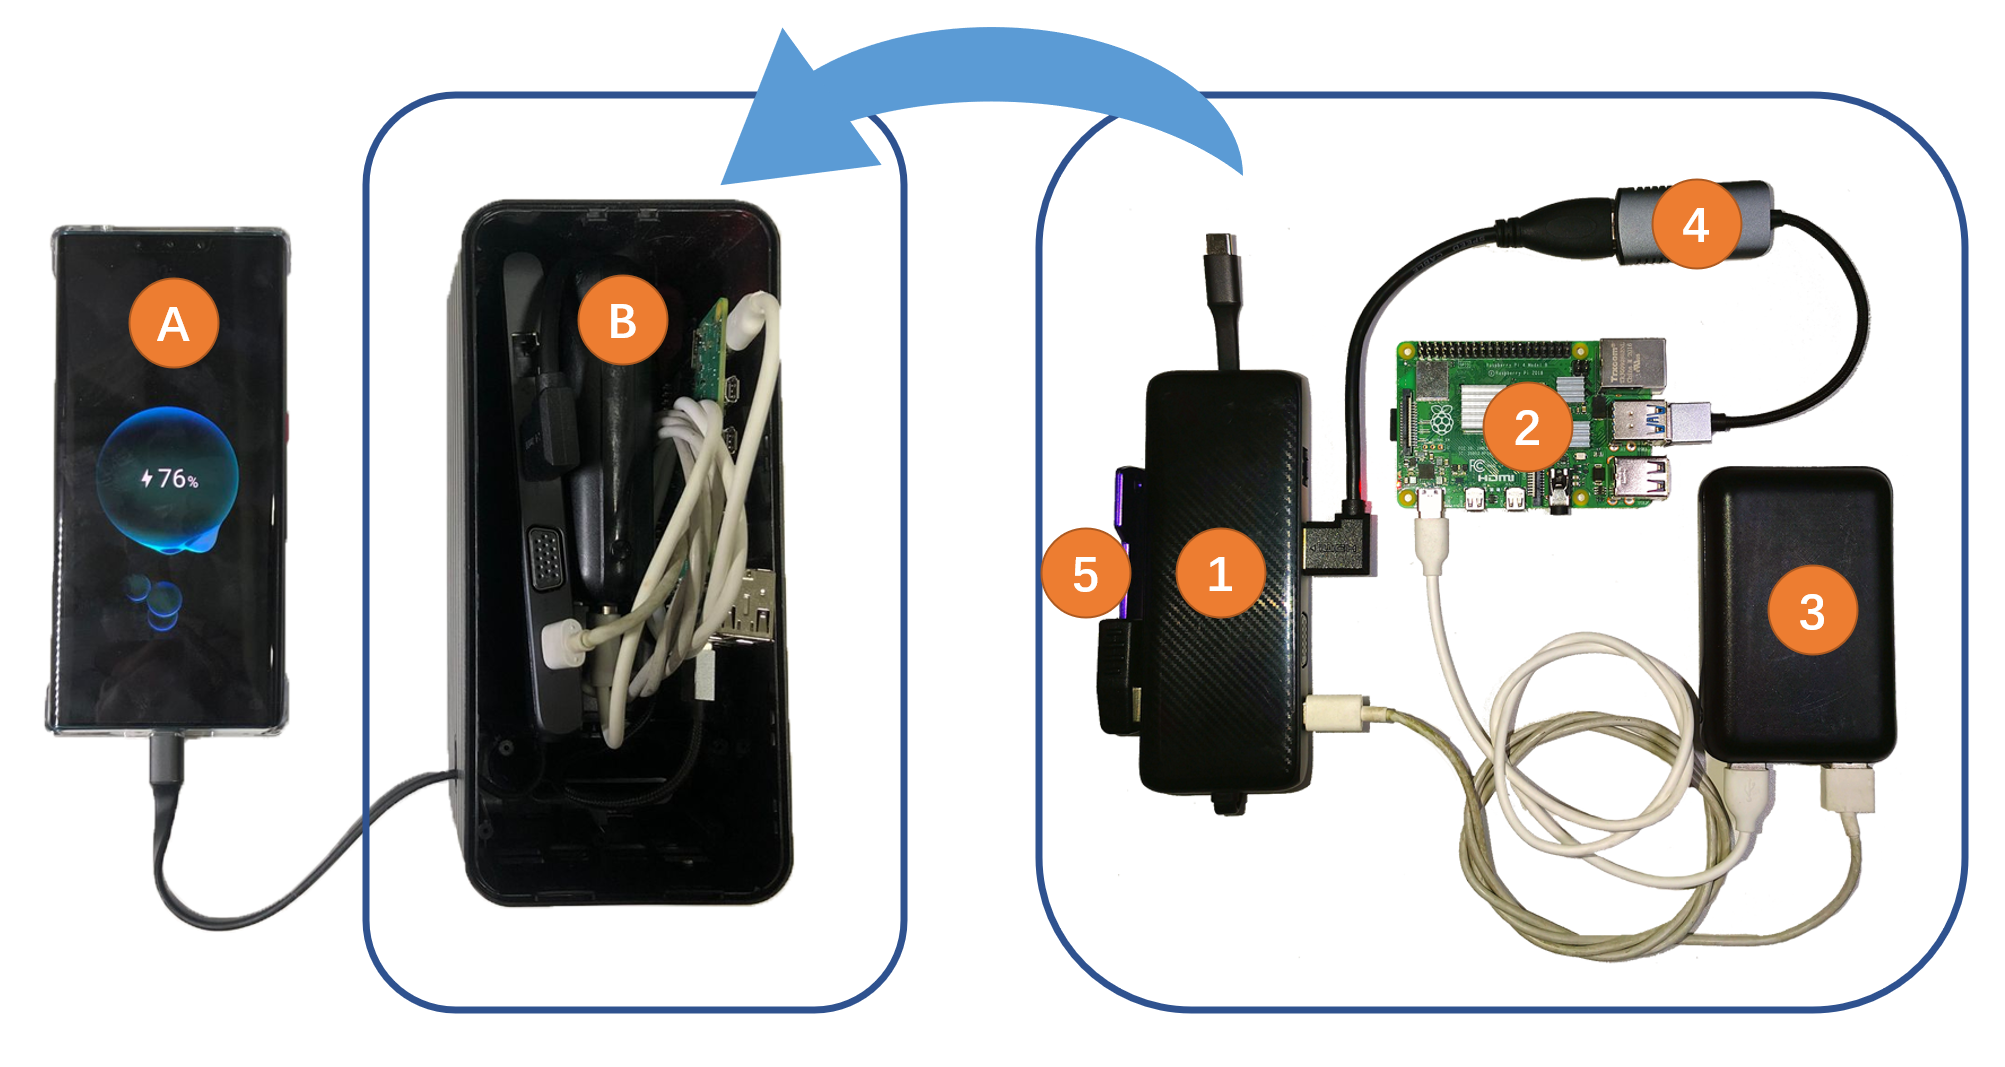
\includegraphics[width=.98\linewidth]{./Figs/armory_all.png}\\
	\begin{tabular}{ll}
	\circled[text=white,fill=myblue]{\scriptsize{A}} Victim's Device    &\circled[text=white,fill=myblue]{\scriptsize{B}}~\tool\\
	\circled[text=white,fill=myblue]{\footnotesize{1}} USB 3.x Hub        &\circled[text=white,fill=myblue]{\footnotesize{2}} Raspberry Pi 4B\\
	\circled[text=white,fill=myblue]{\footnotesize{3}} Auxiliary Power Bank &\circled[text=white,fill=myblue]{\footnotesize{4}} Video Capture\\
	\circled[text=white,fill=myblue]{\footnotesize{5}} ATMEGAA32U4 Board
	\end{tabular}


	\caption{\tool Prototype}
	\label{fig:armory}
\end{figure}

\subsection{HID Emulator Mode}

In the experiment of HID emulator mode, we used {Lenovo Xiaoxin Pro 13
2020}, a PC in Windows 10/Ubuntu OS with two USB Type-C interfaces as the
target device.  During this experiment, \tool disguised itself as a normal
keyboard and a home-brewed version of GoodUSB~\cite{tian2015defending} is
deployed to test the defense-bypassing. We have tried to deploy the original
GoodUSB on the target device; as the GoodUSB is proposed in 2015, the code is
outdated and cannot be executed at target device; so we have to home-brew a similar
defense mechanism based on its paper~\cite{tian2015defending}.  In the
beginning, our home-brewed version of GoodUSB asked the victim to manually complete
a CAPTCHA to authorize the new USB device, a.k.a our \tool. 
%But at this time,
%by the design of GoodUSB, 
%\fengwei{The following sentence is hard to
%understand.}\hongyi{Fixed, removed redundant description} 
However, our attack can enter keystrokes to complete the
CAPTCHA with the video stream by \tool. Up
to this point, the bypass of defense like GoodUSB is completed and our \tool
becomes a trusted device. Next, our
\tool works similar to the original BadUSB, inserting keystrokes to perform
arbitrary execution on the laptop. We tested three scripts, ranging from
reverse shell backdoor to malware payload execution, all of which resulting in
success. With this experiment, we have demonstrated the defense-bypassing is successful
using \tool.
%This also warned us that we need more thorough defense against such BadUSB
%attack.



\subsection{Video Capture Mode}

During the experiment of privacy extraction via our video capture mode, we chose \textit{HUAWEI P30}, a
smartphone in EMUI 9.1 (Android 9.0 based) with a USB Type-C interface, as the
target device.  In the privacy extraction experiment, \tool passively captured video
from the victim's device and used \textit{OpenCV} to identify the sensitive
information from the video stream.  When the victim viewed text or photos with
text, \tool used the techniques of Optical Character Recognition (OCR) \fengwei{do we need a reference for OCR?} to
extract text from corresponding video frames. In this experiment, the attacker had
successfully extracted text like name, address, ID number, and other sensitive
personal information. We also tested the payment code extractor, which enables
an attacker to identify payment code in the video stream and perform transactions
without the password. As this is also a part of our case study, more details about
the extracted sensitive data can be found in Section~\ref{subsec:case_study} and
Table~\ref{table:information_extracted}.

%\fengwei{I don't understand the following sentence. Both modes need to capture
%the video stream. Don't understand why it is more power-efficient.}
%\hongyi{Reasonable, changed to other advantage}
Note that the video capture mode only needs to
process the victim's video stream locally, it does not need to transmit the real-time video back to the attacker, which is needed when the network connection between \tool and the attacker is not stable. 
%This mode is useful when there is no stable network connection between \tool and the attacker.

\subsection{Fully Control Mode}
%\fengwei{In BadUSB-C section, remote control model is after privacy extraction mode.}

To test the capability of the fully control mode, we chose iPad Pro (3rd
	generation), a tablet in iOS 14.3 with a USB Type-C interface, as the target
device in this experiment.  Besides disguising as normal HID devices like a
conventional BadUSB~\cite{badusb}, \tool also transmitted real-time video
stream from the target device to the attacker via WiFi.  After the connection
establishment, the attacker performed a series of actions to test the capability of
\tool. In the beginning, the attacker accessed the album application on the iPad and
obtained all the photos inside. After that, the attacker sent messages via victim's
account. At last, the attacker performed a transaction using the
financial application. All of these tests resulted in success.

Through this experiment, we have found that with video transmission and mouse
emulation, \tool extensively expanded the attack capability of BadUSB,
especially in mobile devices. In short, we have archived the complete hijack of the victim's
device in this experiment.

\subsection{Case study}
\label{subsec:case_study}
\subsubsection{Background}

We first introduce the technical background of our case study, sharing power
bank service and QR code payment.

\textbf{Sharing Power Bank}.  Sharing power bank provides users with short-term
rental of power banks.  The company deploys power bank stations in the city and
users can rent a power bank from any of the power bank station, charge their
device on the trip, return the rented power bank to the near station, and pay
the rental fee.

For example, Brick~\cite{Brick} is such a power bank sharing service
provider from Sweden. It provides power bank rental service all over Sweden
and is planning on expanding its service around Europe. Moreover, this
service is even more popular in Asia, power bank stations are deployed in
markets, stores, and even newsstands.
%This suggests that this service is becoming more and more common around the global, especially in Asia and Europe.
\shuqing{I think we should paraphrase instead of using the descriptions on the website directly. Just to explain \textbf{what we need}.}

\fengwei{Explain the figure in the text.}
\begin{figure}[t]
	\centering
	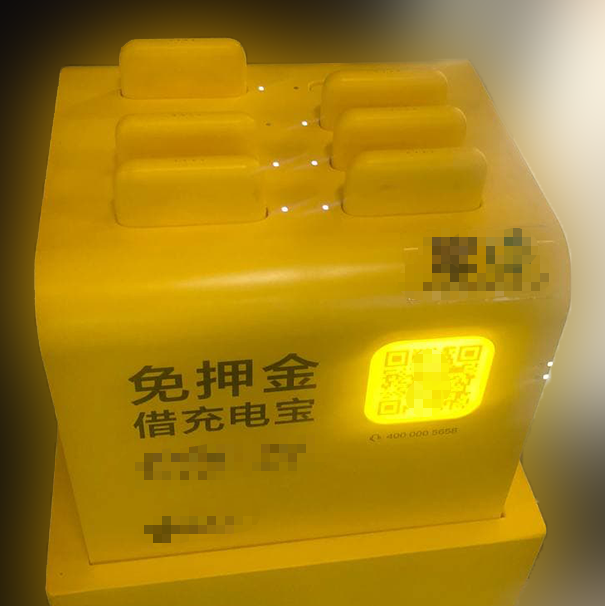
\includegraphics[width=.45 \linewidth, height=.45 \linewidth]{./Figs/PBS_mt.png}
	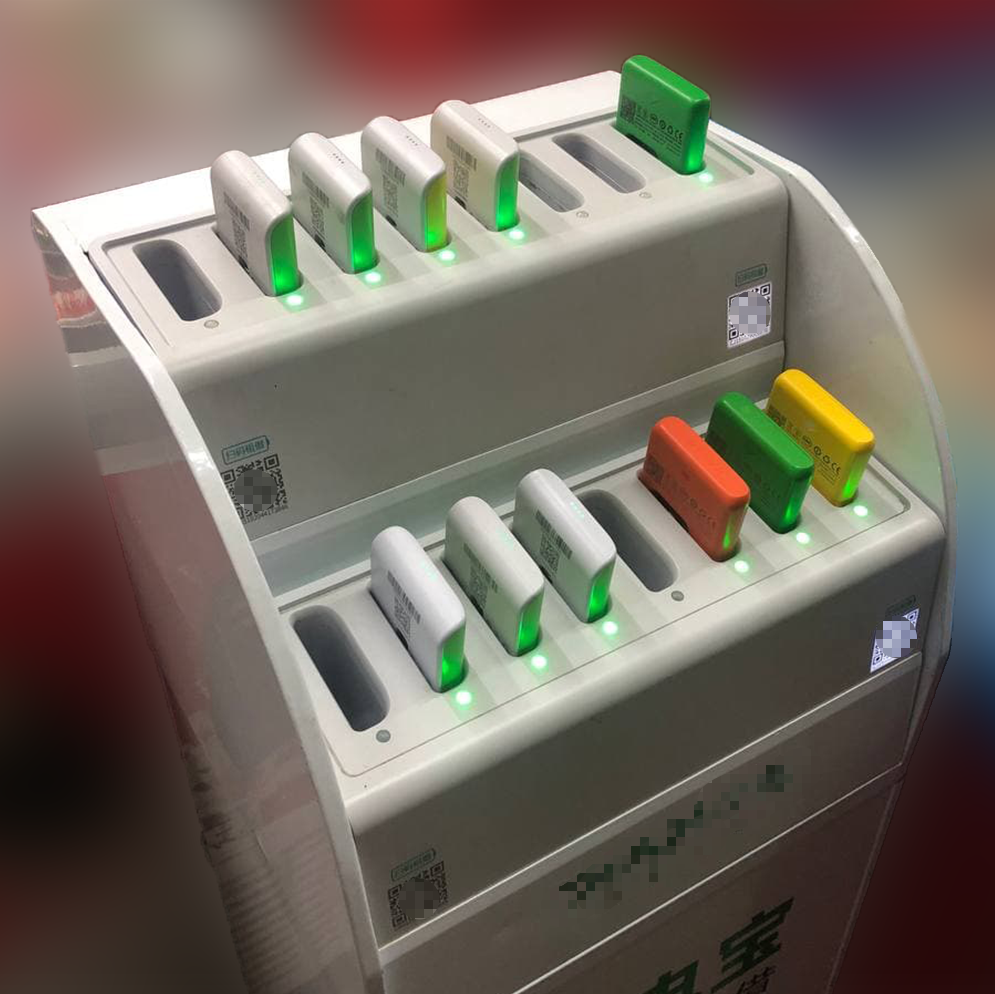
\includegraphics[width=.45 \linewidth, height=.45 \linewidth]{./Figs/PBS_xd.png}
	\caption{Two Power Bank Stations}
	\label{fig:PBS_products}
\end{figure}

\yechang{add hyperlink or reference to Brick's website or Brick App on App Store/Google Play.}

\yechang{Add more examples of power bank sharing to show that it is widely used?}
\shuqing{May use statistics (instead of concrete examples) to explain it.}

Not only does sharing power bank provides convenience to users, but it also
brings security issues.  We noticed that most of the power bank stations do not
check the integrity of power banks during the rental process, and users are
hardly cautious to check the power banks when connecting their devices.  An
attacker is able to tamper rented power banks and return them to a power bank
station causing a potential threat to subsequent users.


\textbf{QR Code Payment}.
QR code payment is a new type of payment method that is popular in Asia. Its most well-known cases are WeChat Pay~\cite{Wechat-pay} and Alipay~\cite{AliPay}. QR code payment provides merchant and client a convenient way of offline payment while ensuring equivalent security as the credit card.
As illustrated in Figure~\ref{fig:qr_payment_procedure}, QR code payment is typically performed in the following steps:
\ding{182} The client presents the payment QR code on the mobile device to the merchant.
The QR code is encoded with a globally unique ID to identify the client's account.
\ding{183} The merchant scans the payment QR code and charges the corresponding amount of money.
By presenting this QR code, the client authorizes the proceeding transaction.
\ding{184} After confirmation, the payment service provider proceed with this transaction and return the payment result to both the merchant and the client.
\shuqing{I think this paragraph can be shorter. No need to explain so many details.}
\hongyi{Dont know how to be more concise.}

\begin{figure}[t]
	\centering
	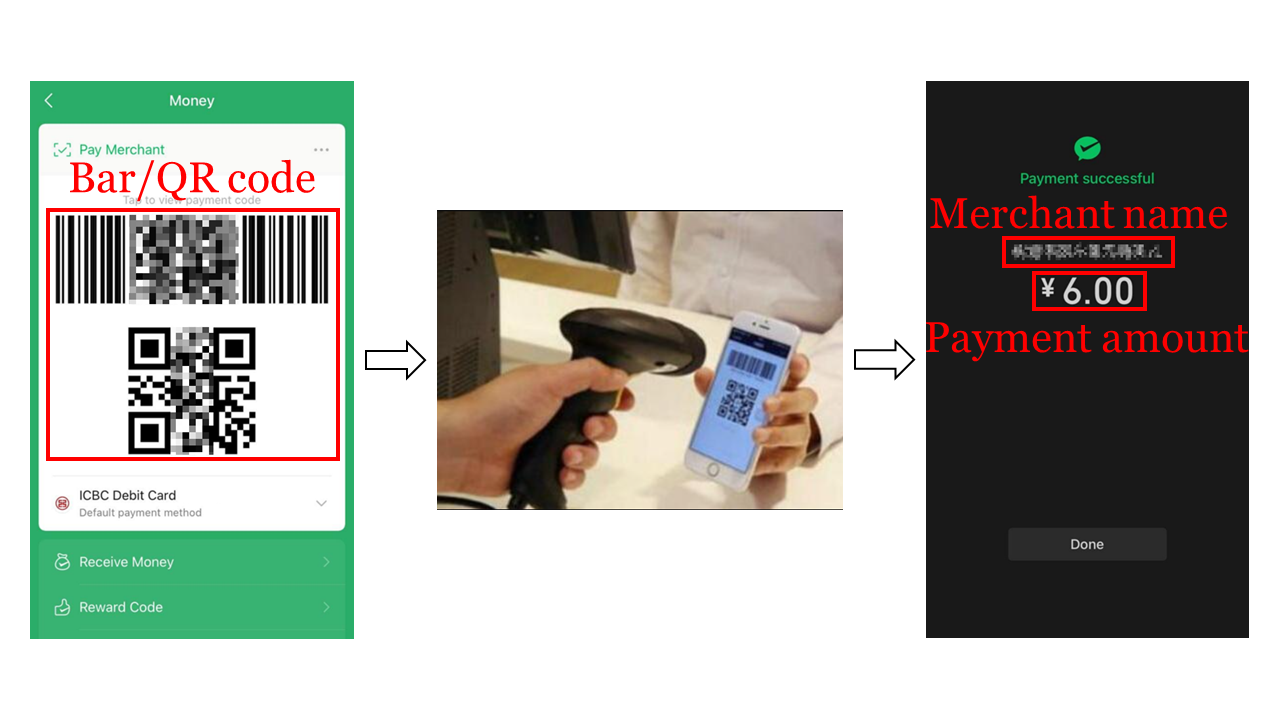
\includegraphics[width=\linewidth]{./Figs/qr_code_payment.png}
	\caption{Bar/QR Code Payment Procedure}
	\label{fig:qr_payment_procedure}
\end{figure}


In the real-world scenario, some payment service providers use special rules
for micropayment purchases.  A micropayment is pre-determined by the payment
service provider with thresholds in the user agreement.  For example, WeChat
Pay~\cite{Wechat-pay} regards transaction under USD \textdollar 154 as
micropayments.  Different from a typical payment procedure, when micropayments
are made, confirmations can be applied automatically without clients'
permission which aims to provide convenience to both merchant and client.  If a
victim's payment code is leaked to the attackers, they can use that code to
authorize multiple micropayments without permission.  In order to prevent such
cases, both WeChat Pay~\cite{Wechat-pay} and Alipay~\cite{AliPay} has designed a refreshing mechanism for the
payment code, which is to refresh the QR code every minute. This is sufficient
to stop an attack like sneak shots but unable to stop a real-time attack like our
\tool.  In summary, the payment QR code is highly sensitive on users' devices
and our following case study is about how to obtain this code using an
attacker-crafted power bank via \tool.

\subsubsection{Attack Scenario}

In this part, we will introduce a real-life attack scenario to show that our
\tool is a practical offensive tool.  This scenario can be decomposed into the
following steps.

\begin{enumerate}[I. ]
	\item The attacker rents a power bank from one of the power bank stations and replaces the internal components with \tool.
	\item After the modification, an attacker-crafted power bank is returned to a rental station in a crowded area like an airport or railway station, which increases the probability of success.
	\item a user borrows the modified power bank and connects it to her own device, becoming the victim of \tool.
	\item The attacker now has complete control over the victim and can perform various attacks using different modes.
\end{enumerate}

Here we summarize the possible threats toward user under different modes. \hongyi{Better way to express this?}
First, under scripting mode, the attacker is able to implant malware and backdoor script into victims' devices. Moreover, using privacy extraction mode, once the victims access their private data like QR payment  code or album, their private data will be immediately transmitted via \tool to the attacker. Lastly, with remote control mode, the attacker has complete control over the victims' device and can do anything they want.

\shuqing{Background is longer than real user study.}
As the functionality and effectiveness of the scripting mode and the remote control mode are rather clear, the former works similar to the original BadUSB, the latter hijacks the victim's device completely.\hongyi{I dont know if it's a good enough reason}
Here we only validate the usability of privacy extraction mode and conducted a user study.
We invited 10 volunteers to participate, who are unconscious of \tool details.
Before the experiment, we disclose to the volunteers how their data might be used and request permission from both the volunteers and the institutional ethics review boards.
During the experiment, volunteers took turns to use their phones for half an hour with \tool connected, which are considered as a normal power bank.
To obtain data close to real life, they are requested to use phones just like when they use the shared power bank outside.
After the experiment, we introduced to them our attack, analyze the screen recordings together to make sure their personal data is not at risk.
\shuqing{Do we need to mention that agreement the conference required here?}
\hongyi{I'm also quite concern about this.}


\subsubsection{Result}
After collecting the videos, we analyzed the video both automatically and manually.
During the automatic analysis, we used scripts to perform OCR recognition for each frame in the recorded video and stored all of the OCR results in a database.
At last, there are 94058 pieces of data collected among 10 volunteers.
\shuqing{The data may need to be updated.}
With these results, we could learn what content the victim was browsing.
Additionally, some keywords such as \textit{account, username, and password} often appear with users' input data because they are often used as labels of input boxes.
Such keywords are more likely to lead us to user-specific data.
For example, when we searched with \textit{account} as a keyword, victim's accounts can be found in the database, as shown in the Table~\ref{tab:ocr_keyword_example}.
\shuqing{Statistics.}
The frame number is the position of this frame in the recorded video, which indicates a target for manual analysis for further data extraction.

\begin{table*}[t]
	\centering
	\begin{tabular}{|l|l|l|l|}
		\hline
		Keyword  & Text                                                                                                                          & Name                           & Frame Number \\ \hline
		username & X 8B cas.******.edu.cn Username: 11****18 Password:                                                                           & \textless{}user1\textgreater{} & 385          \\ \hline
		username & Login Weibo Login with SMS and verification code ...... +86 151****4587 & \textless{}user5\textgreater{} & 1947         \\ \hline
		username & QQ 14*****50| Login with phone number New user registration 2345678 9 0                                                       & \textless{}user3\textgreater{} & 4308         \\ \hline
		username & connect to *** username h*****l Save account information Open VPN.....                                                        & \textless{}user6\textgreater{} & 7925         \\ \hline
		+86      & Login with phone number ...... +86 186****2483 |                                                                              & \textless{}user1\textgreater{} & 313          \\ \hline
	\end{tabular}
	\linebreak
	\caption{Example of searching OCR results with some keywords}
	\label{tab:ocr_keyword_example}
\end{table*}


In the manual analysis, we replayed the recorded video and extracted sensitive information.
The data we collected are listed in Table~\ref{table:information_extracted}.
Accounts of internet applications such as Apple, iCloud, Facebook, Twitter, etc. can be obtained.
Moreover, all of the typing inputs on the virtual keyboard, including the system keyboard and the built-in security keyboard of the financial applications, can be clearly recorded.
We can obtain the plain text of passwords such as WiFi passwords.
Furthermore, the received SMS verification code (usually used to confirm real-name authentication) can be obtained when it appears in the top notification bar.

In summary, though we can't directly obtain the user's password on the lock screen, we can still check all of the information presented on the screen, extract private information including but not limited to social accounts, bank accounts, personal financial situation, etc., if the user unconsciously unlocks the screen.
It is worth mentioning that, those \textit{secure keyboards} built in some financial apps just disrupt keyboard sequences, they can't prevent attacks similar as \tool.

\begin{table*}[t]
	\centering
	\begin{tabular}{|c|c|c|c|c|}
		\hline
		Application Column  & Application & Private information leaked                       \\
		\hline
		Finance App         & Alipay      & Alipay account, personal assets(blance)          \\
		\hline
		Social  Finance App & WeChat      & WeChat account, blance, chat history             \\
		\hline
		Social App          & QQ          & QQ account, interpersonal nexus, chat history    \\
		\hline
		Social App          & Twitter     & Twitter account, interpersonal nexus             \\
		\hline
		Social App          & Gmail       & Gmail account, mail records                      \\
		\hline
		Finance App         & ICBC        & ICBC account, password, personal assets(blance)  \\
		\hline
		Finance App         & Paypal      & Paypal account, blance, bank accounts            \\
		\hline
		Tool                & Chrome      & Sites visited                                    \\
		\hline
		Tool                & Health      & personal physical metrics      					 \\
		\hline
	\end{tabular}
	\linebreak
	\caption{Information extracted}\shuqing{Compress.}
	\label{table:information_extracted}
\end{table*}

\section{Countermeasures}
\label{sec:countermeasures}
Authorization mechanism like GoodUSB\cite{tian2015defending} has been proposed as a countermeasure against BadUSB attack. But as mentioned in Section~\ref{sec:badusb} and Section~\ref{sec:experiment}, GoodUSB relies on internal display to request for authorization, which can be hijacked by our \tool. Hence, GoodUSB is indeed a great defense against traditional BadUSB attack but no defense at all for our \tool. Here we discuss some effective countermeasures against \tool.

\textbf{External Hardware Authorization.}
One possible countermeasure is to introduce external hardware completing the authorization process. Contrary to the GoodUSB, USBCheckIn\cite{usbcheckin} adopts a dedicated hardware between the host and device. When a device is plugged in, the authorization will be complete on the dedicated hardware instead of internal display, preventing the host from being hijacked. Though USBCheckIn is a adequate defense against \tool, the external hardware brings additional cost and inconvenience, especially for mobile device.

\textbf{Isolated UI Rendering}
During our experiment, we noticed that \tool is actually unable to redirect out the locking screen keyboard from the iPad OS. Instead, the keyboard is only available on the internal display. However, this defense is only enabled on the locking screen keyboard, other virtual keyboard is still vulnerable to our \tool. This mechanism has inspired us to propose a new defense against our \tool. If the OS provider like Apple/Google can implement a more generalized \emph{isolated UI rendering} that allows developer to decide whether a content is ``sensitive'' and where it should be rendered. To better illustrate this countermeasure idea, we drew the Figure~\ref{fig:isolated_ui}. In that figure, the password keyboard is set to be ``sensitive'' component while the other parts of the UI is not. Thus the renderer will only render the password keyboard on the trusted internal display and prevent untrusted external display like \tool to obtain sensitive data. We believe this is a promising way to defend users from attack like juice filming and our \tool.
\begin{figure}[t]
	\centering
	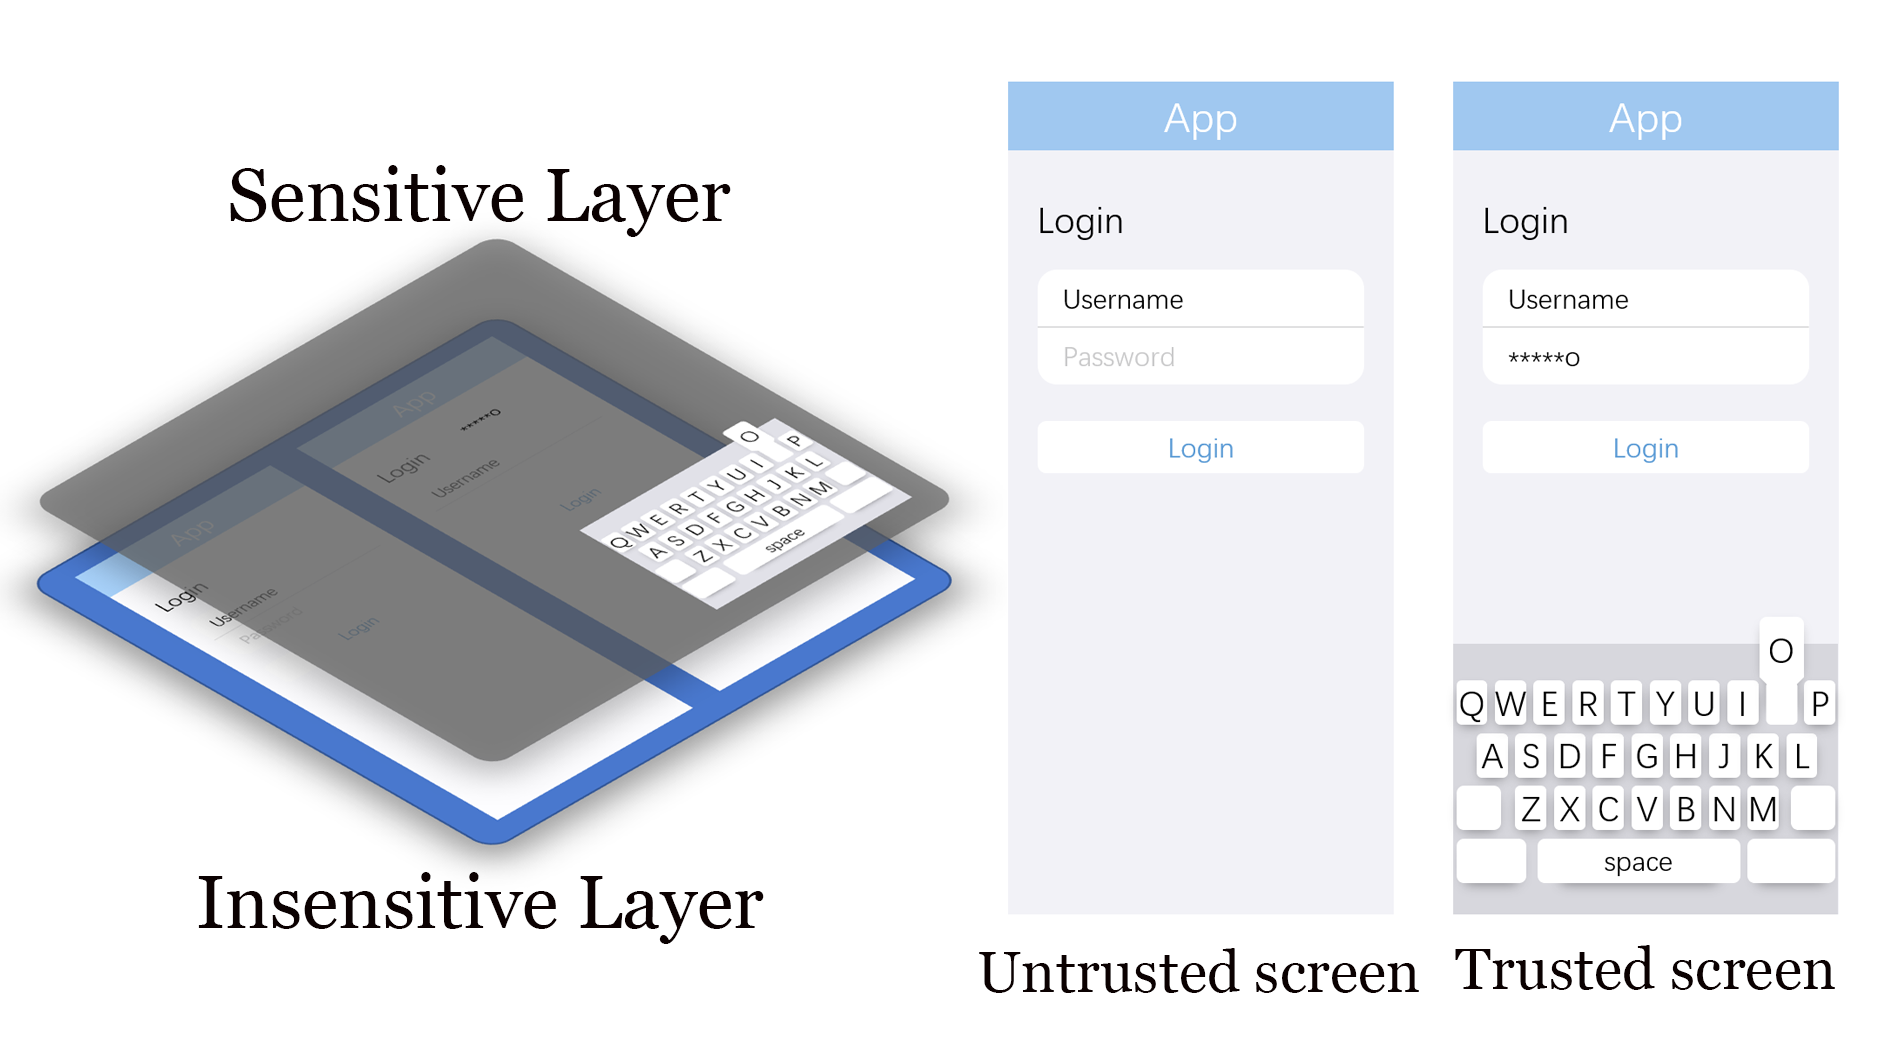
\includegraphics[width=\linewidth]{./Figs/isolated_ui.png}
	\caption{Isolated UI Rendering}\shuqing{Maybe we can increase the font?}
	\label{fig:isolated_ui}
\end{figure}

\textbf{Distrust-by-Default.}
Most security issues of USB protocol is due to its \textit{trust-by-default} policy. \tool also relies on this feature to work. Hence if we reject all \textit{unauthorized} device, \tool and other many USB attacks will fail. It is worth mentioning here that \textit{distrust-by-default} policy is not the same as GoodUSB\cite{tian2015defending}. GoodUSB relies on the \textit{unauthorized} device to complete its own authorization, while in this strict policy, users have to use an \textit{authorized} device. Though \textit{distrust-by-default} policy effectively prevents these attack, this also causes considerable inconvenience for users. For example, when there is no other \textit{authorized} device plugged, it is impossible for user to complete the authorization in the first place. Thus this strict policy is far from optimal in most use cases.
\section{Discussion}
\label{sec:discussion}

\subsection{Limitation}
There exist multiple limitations of \tool.
To begin with, \tool can only gain the information and control access of the host itself instead of external hardware.
Consequently, as we introduced in the Section\ref{sec:countermeasures}, \tool can hardly bypass the defence approaches which use external hardware for authorization.
Moreover, most of the devices will prompt users to give authentication to the USB devices or select one of the functional modes after they are plugged in.
Though some of such prompts are not conspicuous for non-experts, especially when \tool is concealed within other functional hardware such as portable battery \shuqing{If there is experiment, add it here.}, the probability whether users could get aware that something unusual happens will increase with the existence these prompting messages.

\subsection{Impact}
\shuqing{Left after experiment to finish. Will discuss from different modes and application scenarios.}

\section{Conclusion}
\label{sec:conclusion}
\outline{Conclusion}

Leveraging the new features of \ac{USB} 3.x~\cite{usb30,usb31,usb32}, we explore a
new attack scheme named \tool and three attack modes. Each of these three modes
has its own strength and use scenarios. The \ac{HID} Emulation mode largely extends the
original BadUSB. The video capture mode proved practical and powerful, as it extracts
victim's sensitive information in a stealthy way. The full control mode
achieves the complete hijack of the target device, allowing us to perform various
types of subsequent attacks. By experimenting \tool with mobile phones, tablets,
and PCs, we further test its ability under different modes. In our experiment, we
obtain and analyze video stream extracted from 11 applications with \tool,
which demonstrates its capability in a simulated real-life scenario. In the end, we
propose a new defense scheme named \textit{isolated UI rendering}, which can
effectively stop attacks with \tool.
As for future work, we will further explore the potential of \textit{isolated UI
rendering} and implement it on a customized operating system. Moreover, we also
hope to lower the power consumption for network transmission in \tool to make
it more practical.

\section{Responsible Disclosure}
Responsible disclosure have already been carried out, we have contacted HUAWEI and Apple through proper channels. We received response from HUAWEI on March \nth{7} and discussed the mitigation plan on March \nth{10} while Apple has not responded yet. HUAWEI security team has confirmed this issue and been working on mitigation. We are actively facilitating their mitigation process and waiting for a fix to be deployed. After the mitigation is deployed, HUAWEI will assign a CVE ID for this vulnerability.

\section{Acknowledgement}
We are very grateful to our shepherd, Michael Schwarz, and the anonymous reviewers for their valuable feedback that improved the paper.

%\input{./Files/acknowledgement.tex}

\bibliographystyle{IEEEtran}
\bibliography{BadUSBC}
\balance


\end{document}
